% CENTRAL OBSERVABILITY DESIGN VISUALS
% Updated companion for central_observability_design.md.
% Compile: pdflatex CENTRAL_OBSERVABILITY_VISUALS.tex (twice)
\documentclass[10pt]{article}
\usepackage[a4paper,landscape,margin=10mm]{geometry}
\usepackage[T1]{fontenc}
\usepackage[utf8]{inputenc}
\usepackage[sc]{mathpazo}
\usepackage{microtype}
\usepackage{tikz}
\usetikzlibrary{arrows.meta,positioning,fit,calc,backgrounds,shapes.geometric,shapes.multipart,decorations.pathreplacing,matrix}
\usepackage{xcolor}
\usepackage{adjustbox}
\usepackage{hyperref}
\hypersetup{hidelinks}
\pagestyle{empty}
\setlength{\parindent}{0pt}

\definecolor{store}{HTML}{EAF0FF}
\definecolor{source}{HTML}{EAF8EC}
\definecolor{writer}{HTML}{FFF0EE}
\definecolor{reader}{HTML}{F6EDFA}
\definecolor{ci}{HTML}{FFF5E6}
\definecolor{external}{HTML}{F4F4F4}
\definecolor{risk}{HTML}{FFE3E3}
\definecolor{good}{HTML}{E2F5E7}
\definecolor{policy}{HTML}{E8F7F5}
\definecolor{ink}{HTML}{263238}
\definecolor{muted}{HTML}{607D8B}
\definecolor{red}{HTML}{B54A4A}
\definecolor{purple}{HTML}{7A4E9B}
\definecolor{orange}{HTML}{B56A24}
\definecolor{green}{HTML}{39784A}
\definecolor{blue}{HTML}{3F6FB5}

\tikzset{
  >=Latex,
  every node/.style={font=\small,text=ink},
  box/.style={draw=ink!65,rounded corners=2.5pt,fill=store,minimum height=11mm,minimum width=34mm,align=center,inner sep=4pt},
  sourcebox/.style={box,fill=source,draw=green!70},
  writerbox/.style={box,fill=writer,draw=red!70},
  readerbox/.style={box,fill=reader,draw=purple!70},
  cibox/.style={box,fill=ci,draw=orange!75},
  extbox/.style={box,fill=external,dashed},
  policybox/.style={box,fill=policy,draw=green!70},
  riskbox/.style={box,fill=risk,draw=red!80},
  goodbox/.style={box,fill=good,draw=green!75},
  tinybox/.style={draw=ink!55,rounded corners=2pt,fill=white,align=center,inner sep=3pt,font=\footnotesize},
  state/.style={draw=ink!65,rounded corners=6pt,fill=store,minimum width=28mm,minimum height=10mm,align=center},
  terminal/.style={state,fill=good,draw=green!75},
  badstate/.style={state,fill=risk,draw=red!80},
  arrow/.style={->,very thick,draw=ink!75},
  async/.style={->,thick,dashed,draw=purple},
  write/.style={->,very thick,draw=red},
  policyarr/.style={->,very thick,draw=green},
  effect/.style={->,very thick,draw=orange},
  fail/.style={->,very thick,dashed,draw=red},
  note/.style={draw=ink!30,rounded corners=2pt,fill=white,align=left,inner sep=5pt,font=\footnotesize,text width=70mm},
  pill/.style={draw=ink!45,rounded corners=7pt,fill=white,inner xsep=6pt,inner ysep=2pt,font=\footnotesize\bfseries},
  label/.style={font=\footnotesize,align=center,fill=white,inner sep=1.5pt},
}
\newcommand{\code}[1]{\texttt{\detokenize{#1}}}
\newcommand{\pagehead}[2]{%
  \begin{minipage}[t]{0.73\linewidth}
    {\Large\bfseries #1}\\[-1mm]
    {\small\color{muted}#2}
  \end{minipage}\hfill
  \begin{minipage}[t]{0.25\linewidth}\raggedleft
    {\footnotesize Central observability - reviewed design}\\
    {\scriptsize dev/query branches, July 2026}
  \end{minipage}
  \vspace{3mm}\hrule\vspace{4mm}
}
\newcommand{\legend}{%
\tikz[baseline=-0.7ex]\node[sourcebox,minimum width=7mm,minimum height=4mm,inner sep=1pt]{}; sources\quad
\tikz[baseline=-0.7ex]\node[writerbox,minimum width=7mm,minimum height=4mm,inner sep=1pt]{}; writers\quad
\tikz[baseline=-0.7ex]\node[policybox,minimum width=7mm,minimum height=4mm,inner sep=1pt]{}; policy/contract\quad
\tikz[baseline=-0.7ex]\node[box,minimum width=7mm,minimum height=4mm,inner sep=1pt]{}; store\quad
\tikz[baseline=-0.7ex]\node[readerbox,minimum width=7mm,minimum height=4mm,inner sep=1pt]{}; readers\quad
\tikz[baseline=-0.7ex]\node[cibox,minimum width=7mm,minimum height=4mm,inner sep=1pt]{}; CI/automation
}

\begin{document}

% =====================================================================
% PAGE 1
% =====================================================================
\pagehead{P1. One store, two writer lanes, one contract}
{Debug Console uploads and perftest push write the same SQL Server projection. Files remain ground truth; central is shared evidence.}
\legend\par\vspace{4mm}

\begin{adjustbox}{max width=\linewidth,max height=0.82\textheight,center}
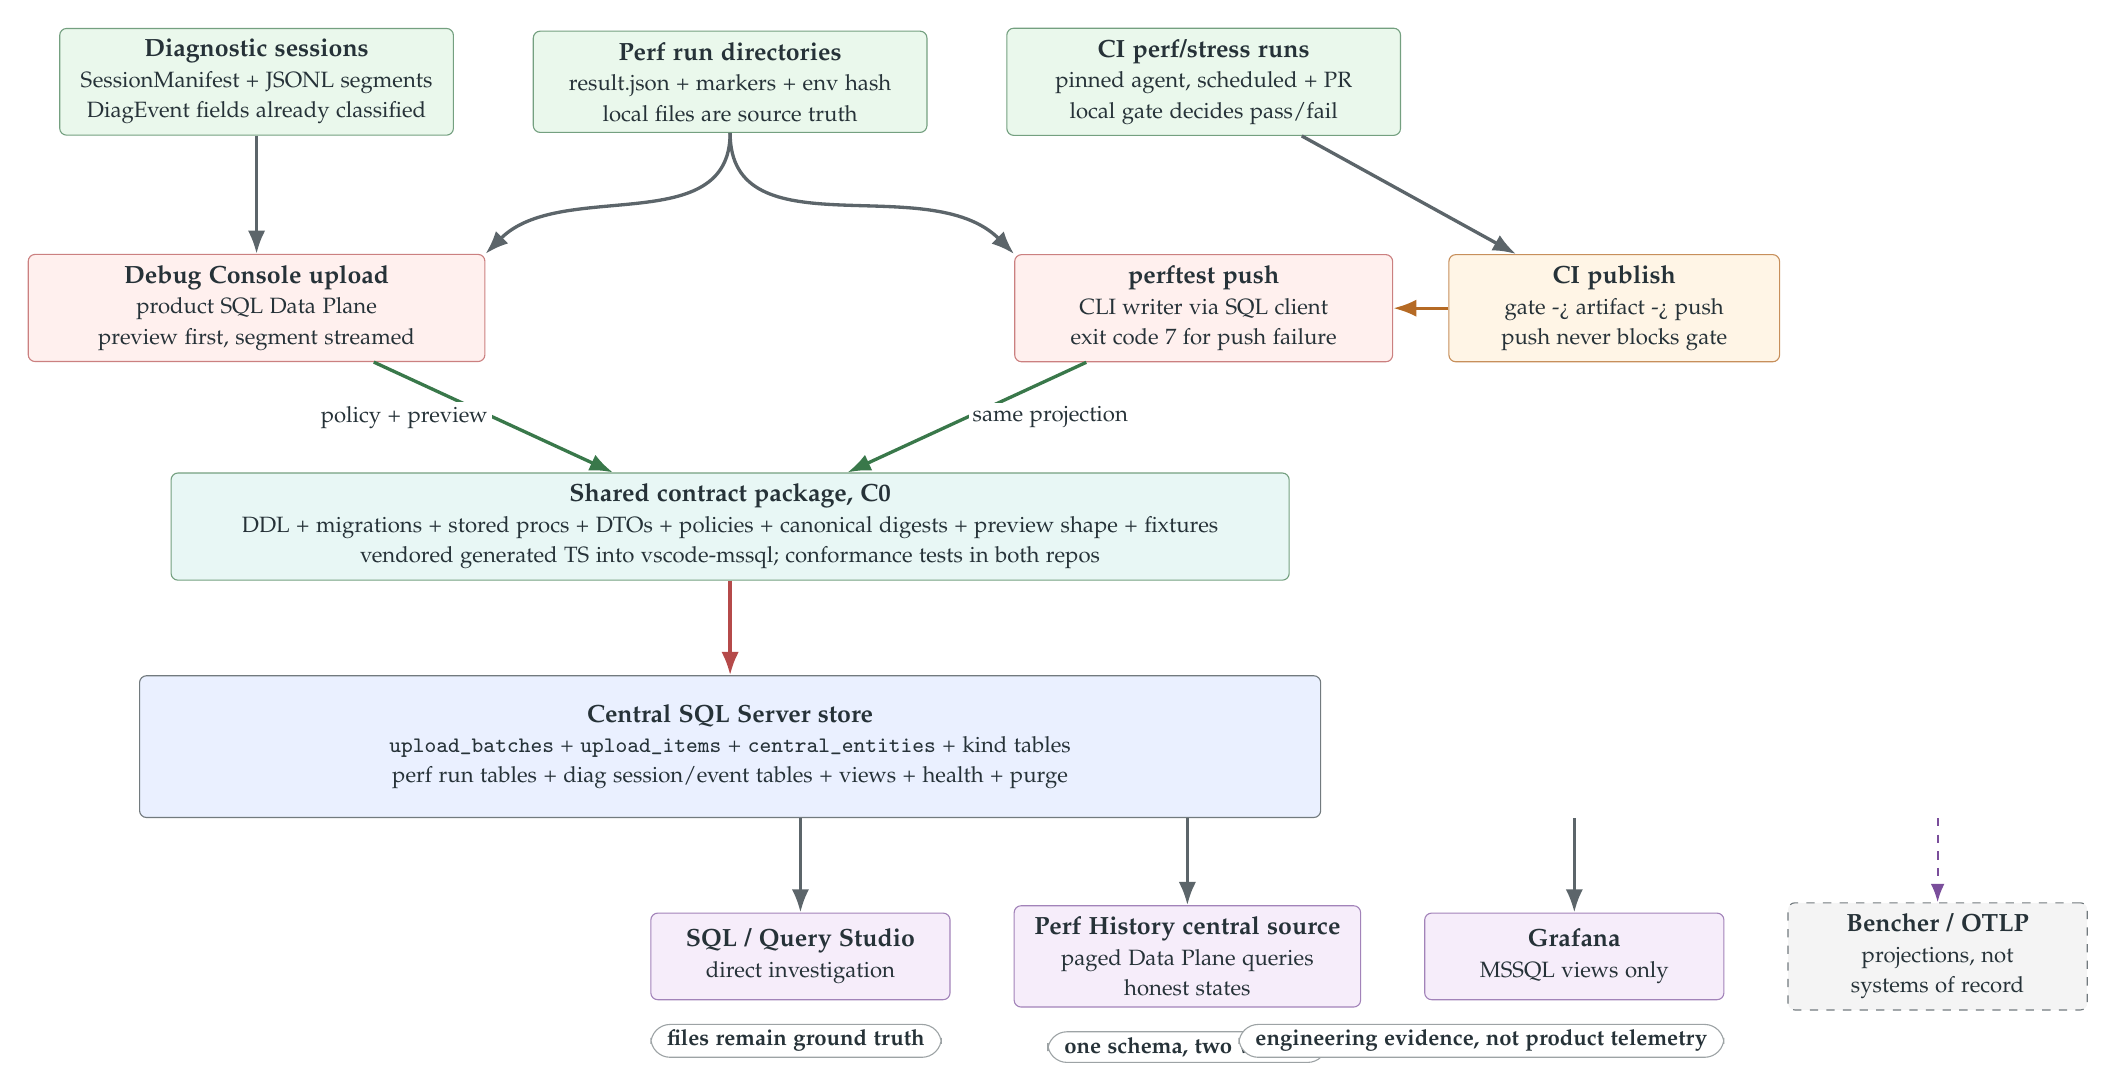
\begin{tikzpicture}[node distance=8mm and 10mm]

\node[sourcebox,minimum width=50mm] (sessions)
{\textbf{Diagnostic sessions}\\\footnotesize SessionManifest + JSONL segments\\\footnotesize DiagEvent fields already classified};
\node[sourcebox,minimum width=50mm,right=of sessions] (runs)
{\textbf{Perf run directories}\\\footnotesize result.json + markers + env hash\\\footnotesize local files are source truth};
\node[sourcebox,minimum width=50mm,right=of runs] (ciRuns)
{\textbf{CI perf/stress runs}\\\footnotesize pinned agent, scheduled + PR\\\footnotesize local gate decides pass/fail};

\node[writerbox,minimum width=58mm,below=15mm of sessions] (debug)
{\textbf{Debug Console upload}\\\footnotesize product SQL Data Plane\\\footnotesize preview first, segment streamed};
\node[writerbox,minimum width=48mm,below=15mm of ciRuns] (push)
{\textbf{perftest push}\\\footnotesize CLI writer via SQL client\\\footnotesize exit code 7 for push failure};
\node[cibox,minimum width=42mm,right=7mm of push] (workflow)
{\textbf{CI publish}\\\footnotesize gate -> artifact -> push\\\footnotesize push never blocks gate};

\node[policybox,minimum width=142mm,below=14mm of $(debug.south)!0.5!(push.south)$] (contract)
{\textbf{Shared contract package, C0}\\\footnotesize DDL + migrations + stored procs + DTOs + policies + canonical digests + preview shape + fixtures\\\footnotesize vendored generated TS into vscode-mssql; conformance tests in both repos};

\node[box,minimum width=150mm,minimum height=18mm,below=12mm of contract] (store)
{\textbf{Central SQL Server store}\\\footnotesize \code{upload_batches} + \code{upload_items} + \code{central_entities} + kind tables\\\footnotesize perf run tables + diag session/event tables + views + health + purge};

\node[readerbox,minimum width=38mm,below left=12mm and -28mm of store.south] (sql)
{\textbf{SQL / Query Studio}\\\footnotesize direct investigation};
\node[readerbox,minimum width=44mm,right=8mm of sql] (provider)
{\textbf{Perf History central source}\\\footnotesize paged Data Plane queries\\\footnotesize honest states};
\node[readerbox,minimum width=38mm,right=8mm of provider] (grafana)
{\textbf{Grafana}\\\footnotesize MSSQL views only};
\node[extbox,minimum width=38mm,right=8mm of grafana] (projections)
{\textbf{Bencher / OTLP}\\\footnotesize projections, not\\\footnotesize systems of record};

\draw[arrow] (sessions) -- (debug);
\draw[arrow] (runs.south) to[out=-90,in=45] (debug.north east);
\draw[arrow] (runs.south) to[out=-90,in=135] (push.north west);
\draw[arrow] (ciRuns) -- (workflow);
\draw[effect] (workflow) -- (push);
\draw[policyarr] (debug) -- node[label,left]{policy + preview} (contract);
\draw[policyarr] (push) -- node[label,right]{same projection} (contract);
\draw[write] (contract) -- (store);
\draw[arrow] (store.south -| sql.north) -- (sql.north);
\draw[arrow] (store.south -| provider.north) -- (provider.north);
\draw[arrow] (store.south -| grafana.north) -- (grafana.north);
\draw[async] (store.south -| projections.north) -- (projections.north);

\node[pill,below=3mm of sql.south west,anchor=north west] {files remain ground truth};
\node[pill,below=3mm of provider.south,anchor=north] {one schema, two writers};
\node[pill,below=3mm of grafana.south east,anchor=north east] {engineering evidence, not product telemetry};

\end{tikzpicture}
\end{adjustbox}

\newpage
% =====================================================================
% PAGE 2
% =====================================================================
\pagehead{P2. Contract and ingest protocol}
{The anti-drift mechanism is the contract: both writers project fixtures to the same rows before any feature UI exists.}
\legend\par\vspace{4mm}

\begin{adjustbox}{max width=\linewidth,max height=0.82\textheight,center}
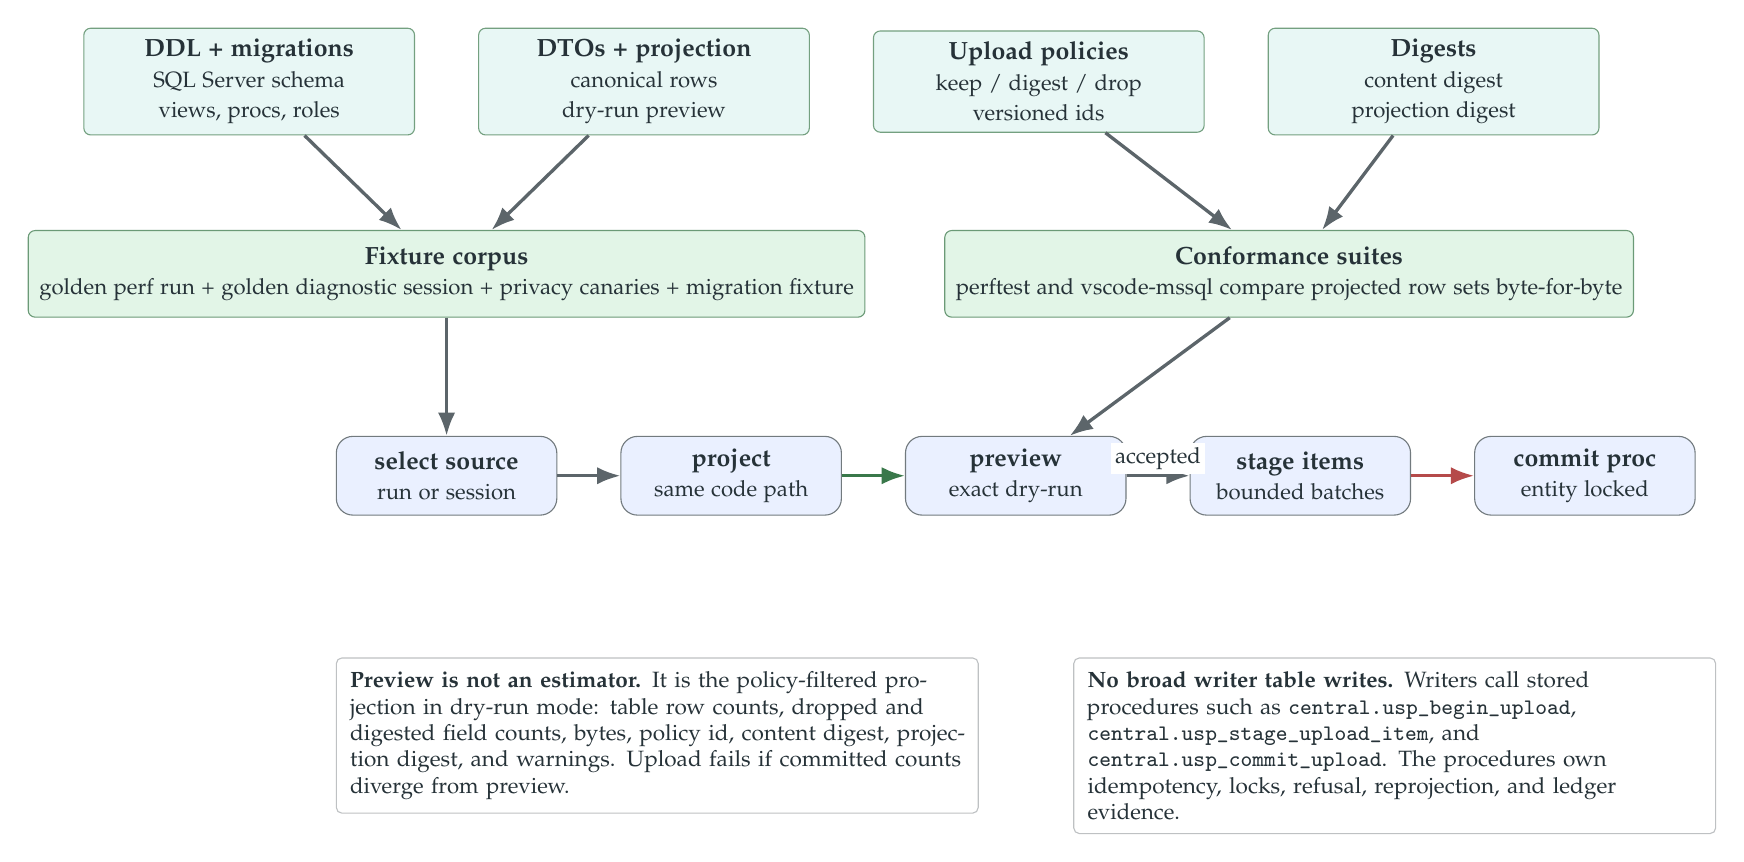
\begin{tikzpicture}[node distance=8mm and 8mm]

\node[policybox,minimum width=42mm] (ddl) {\textbf{DDL + migrations}\\\footnotesize SQL Server schema\\\footnotesize views, procs, roles};
\node[policybox,minimum width=42mm,right=of ddl] (dto) {\textbf{DTOs + projection}\\\footnotesize canonical rows\\\footnotesize dry-run preview};
\node[policybox,minimum width=42mm,right=of dto] (policy) {\textbf{Upload policies}\\\footnotesize keep / digest / drop\\\footnotesize versioned ids};
\node[policybox,minimum width=42mm,right=of policy] (digest) {\textbf{Digests}\\\footnotesize content digest\\\footnotesize projection digest};

\node[goodbox,minimum width=84mm,below=12mm of $(ddl.south)!0.5!(dto.south)$] (fixtures)
{\textbf{Fixture corpus}\\\footnotesize golden perf run + golden diagnostic session + privacy canaries + migration fixture};
\node[goodbox,minimum width=84mm,right=10mm of fixtures] (conf)
{\textbf{Conformance suites}\\\footnotesize perftest and vscode-mssql compare projected row sets byte-for-byte};

\node[state,below=15mm of fixtures] (select) {\textbf{select source}\\\footnotesize run or session};
\node[state,right=of select] (project) {\textbf{project}\\\footnotesize same code path};
\node[state,right=of project] (preview) {\textbf{preview}\\\footnotesize exact dry-run};
\node[state,right=of preview] (upload) {\textbf{stage items}\\\footnotesize bounded batches};
\node[state,right=of upload] (commit) {\textbf{commit proc}\\\footnotesize entity locked};

\draw[arrow] (ddl) -- (fixtures);
\draw[arrow] (dto) -- (fixtures);
\draw[arrow] (policy) -- (conf);
\draw[arrow] (digest) -- (conf);
\draw[arrow] (fixtures) -- (select);
\draw[arrow] (conf) -- (preview);
\draw[arrow] (select) -- (project);
\draw[policyarr] (project) -- (preview);
\draw[arrow] (preview) -- node[label,above]{accepted} (upload);
\draw[write] (upload) -- (commit);

\node[note,below=18mm of select.south west,anchor=north west,text width=78mm] (p2note1)
{\textbf{Preview is not an estimator.} It is the policy-filtered projection in dry-run mode: table row counts, dropped and digested field counts, bytes, policy id, content digest, projection digest, and warnings. Upload fails if committed counts diverge from preview.};

\node[note,right=12mm of p2note1.north east,anchor=north west,text width=78mm] (p2note2)
{\textbf{No broad writer table writes.} Writers call stored procedures such as \code{central.usp_begin_upload}, \code{central.usp_stage_upload_item}, and \code{central.usp_commit_upload}. The procedures own idempotency, locks, refusal, reprojection, and ledger evidence.};

\end{tikzpicture}
\end{adjustbox}

\newpage
% =====================================================================
% PAGE 3
% =====================================================================
\pagehead{P3. Store model: batches, items, entities, and kind tables}
{The draft ledger becomes a stronger ingest spine: attempts are batches; current truth is an entity; analysis lives in kind-specific tables.}
\legend\par\vspace{4mm}

\begin{adjustbox}{max width=\linewidth,max height=0.82\textheight,center}
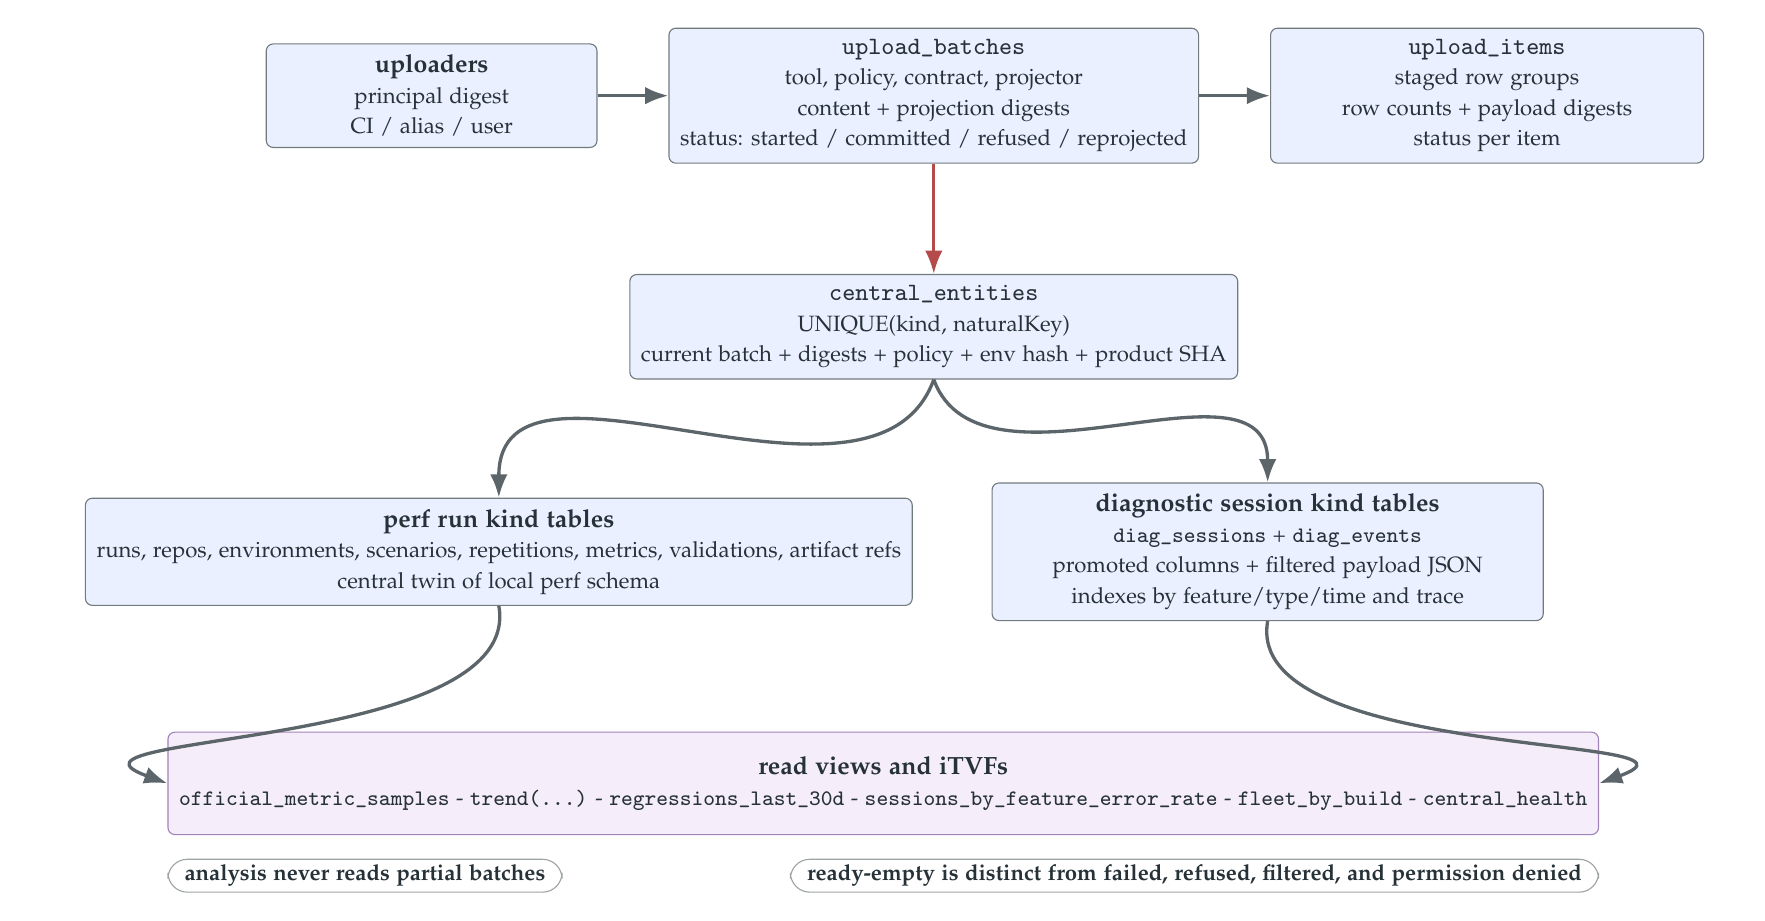
\begin{tikzpicture}[node distance=8mm and 9mm]

\node[box,minimum width=42mm] (uploaders) {\textbf{uploaders}\\\footnotesize principal digest\\\footnotesize CI / alias / user};
\node[box,minimum width=65mm,right=of uploaders] (batches) {\textbf{\code{upload_batches}}\\\footnotesize tool, policy, contract, projector\\\footnotesize content + projection digests\\\footnotesize status: started / committed / refused / reprojected};
\node[box,minimum width=55mm,right=of batches] (items) {\textbf{\code{upload_items}}\\\footnotesize staged row groups\\\footnotesize row counts + payload digests\\\footnotesize status per item};

\draw[arrow] (uploaders) -- (batches);
\draw[arrow] (batches) -- (items);

\node[box,minimum width=72mm,below=14mm of batches] (entities)
{\textbf{\code{central_entities}}\\\footnotesize UNIQUE(kind, naturalKey)\\\footnotesize current batch + digests + policy + env hash + product SHA};
\draw[write] (batches) -- (entities);

\node[box,minimum width=70mm,below left=15mm and -36mm of entities] (perf)
{\textbf{perf run kind tables}\\\footnotesize runs, repos, environments, scenarios, repetitions, metrics, validations, artifact refs\\\footnotesize central twin of local perf schema};
\node[box,minimum width=70mm,right=10mm of perf] (diag)
{\textbf{diagnostic session kind tables}\\\footnotesize \code{diag_sessions} + \code{diag_events}\\\footnotesize promoted columns + filtered payload JSON\\\footnotesize indexes by feature/type/time and trace};

\draw[arrow] (entities.south) to[out=-110,in=90] (perf.north);
\draw[arrow] (entities.south) to[out=-70,in=90] (diag.north);

\node[readerbox,minimum width=150mm,minimum height=13mm,below=15mm of $(perf.south)!0.5!(diag.south)$] (views)
{\textbf{read views and iTVFs}\\\footnotesize \code{official_metric_samples} - \code{trend(...)} - \code{regressions_last_30d} - \code{sessions_by_feature_error_rate} - \code{fleet_by_build} - \code{central_health}};
\draw[arrow] (perf.south) to[out=-80,in=160] (views.west);
\draw[arrow] (diag.south) to[out=-100,in=20] (views.east);

\node[pill,below=3mm of views.south west,anchor=north west] {analysis never reads partial batches};
\node[pill,below=3mm of views.south east,anchor=north east] {ready-empty is distinct from failed, refused, filtered, and permission denied};

\end{tikzpicture}
\end{adjustbox}

\newpage
% =====================================================================
% PAGE 4
% =====================================================================
\pagehead{P4. Privacy and upload policy gate}
{Capture policy controls local collection. Upload policy controls exfiltration. The boundary filters again, and the preview shows the evidence.}
\legend\par\vspace{4mm}

\begin{adjustbox}{max width=\linewidth,max height=0.82\textheight,center}
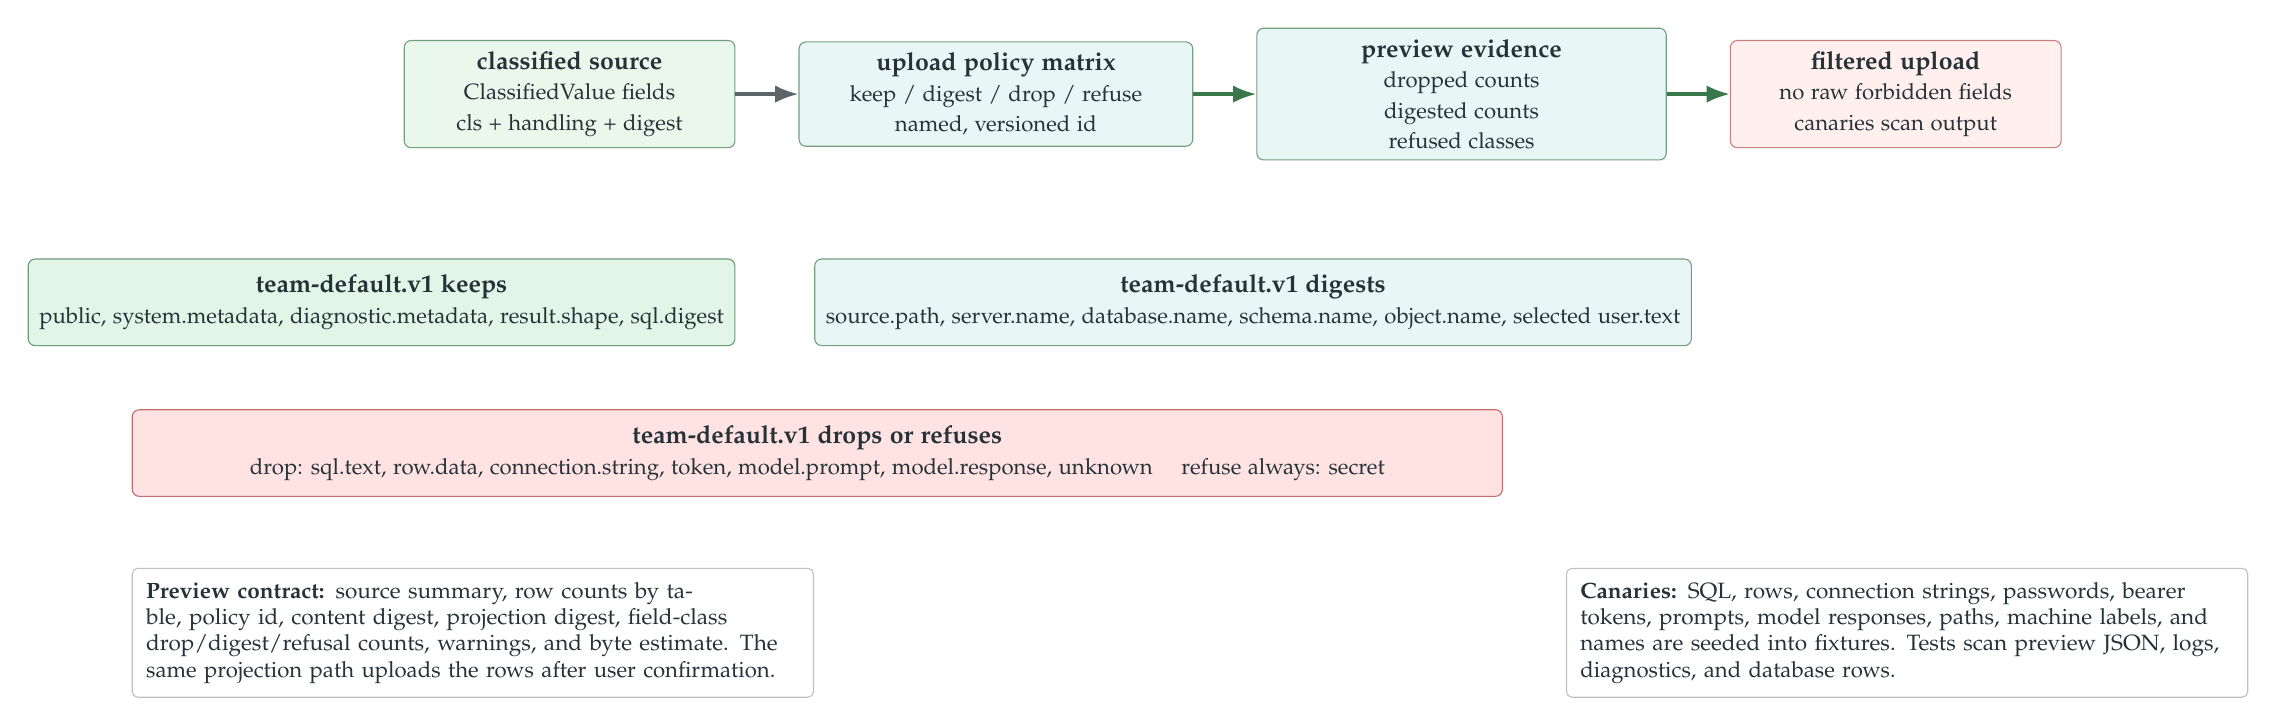
\begin{tikzpicture}[node distance=7mm and 8mm]

\node[sourcebox,minimum width=42mm] (raw) {\textbf{classified source}\\\footnotesize ClassifiedValue fields\\\footnotesize cls + handling + digest};
\node[policybox,minimum width=50mm,right=of raw] (matrix) {\textbf{upload policy matrix}\\\footnotesize keep / digest / drop / refuse\\\footnotesize named, versioned id};
\node[policybox,minimum width=52mm,right=of matrix] (preview) {\textbf{preview evidence}\\\footnotesize dropped counts\\\footnotesize digested counts\\\footnotesize refused classes};
\node[writerbox,minimum width=42mm,right=of preview] (write) {\textbf{filtered upload}\\\footnotesize no raw forbidden fields\\\footnotesize canaries scan output};

\draw[arrow] (raw) -- (matrix);
\draw[policyarr] (matrix) -- (preview);
\draw[policyarr] (preview) -- (write);

\node[goodbox,minimum width=82mm,below=14mm of raw.south east,anchor=north east] (keep)
{\textbf{team-default.v1 keeps}\\\footnotesize public, system.metadata, diagnostic.metadata, result.shape, sql.digest};
\node[policybox,minimum width=82mm,right=10mm of keep] (digest)
{\textbf{team-default.v1 digests}\\\footnotesize source.path, server.name, database.name, schema.name, object.name, selected user.text};
\node[riskbox,minimum width=174mm,below=8mm of $(keep.south)!0.5!(digest.south)$] (drop)
{\textbf{team-default.v1 drops or refuses}\\\footnotesize drop: sql.text, row.data, connection.string, token, model.prompt, model.response, unknown \quad refuse always: secret};

\node[note,below=9mm of drop.south west,anchor=north west,text width=83mm]
{\textbf{Preview contract:} source summary, row counts by table, policy id, content digest, projection digest, field-class drop/digest/refusal counts, warnings, and byte estimate. The same projection path uploads the rows after user confirmation.};

\node[note,right=8mm of drop.south east,anchor=north west,yshift=-9mm,text width=83mm]
{\textbf{Canaries:} SQL, rows, connection strings, passwords, bearer tokens, prompts, model responses, paths, machine labels, and names are seeded into fixtures. Tests scan preview JSON, logs, diagnostics, and database rows.};

\end{tikzpicture}
\end{adjustbox}

\newpage
% =====================================================================
% PAGE 5
% =====================================================================
\pagehead{P5. Writer lanes and failure semantics}
{The CLI and product writers use different transports but the same projection. Central failure is visible evidence, never data loss.}
\legend\par\vspace{4mm}

\begin{adjustbox}{max width=\linewidth,max height=0.82\textheight,center}
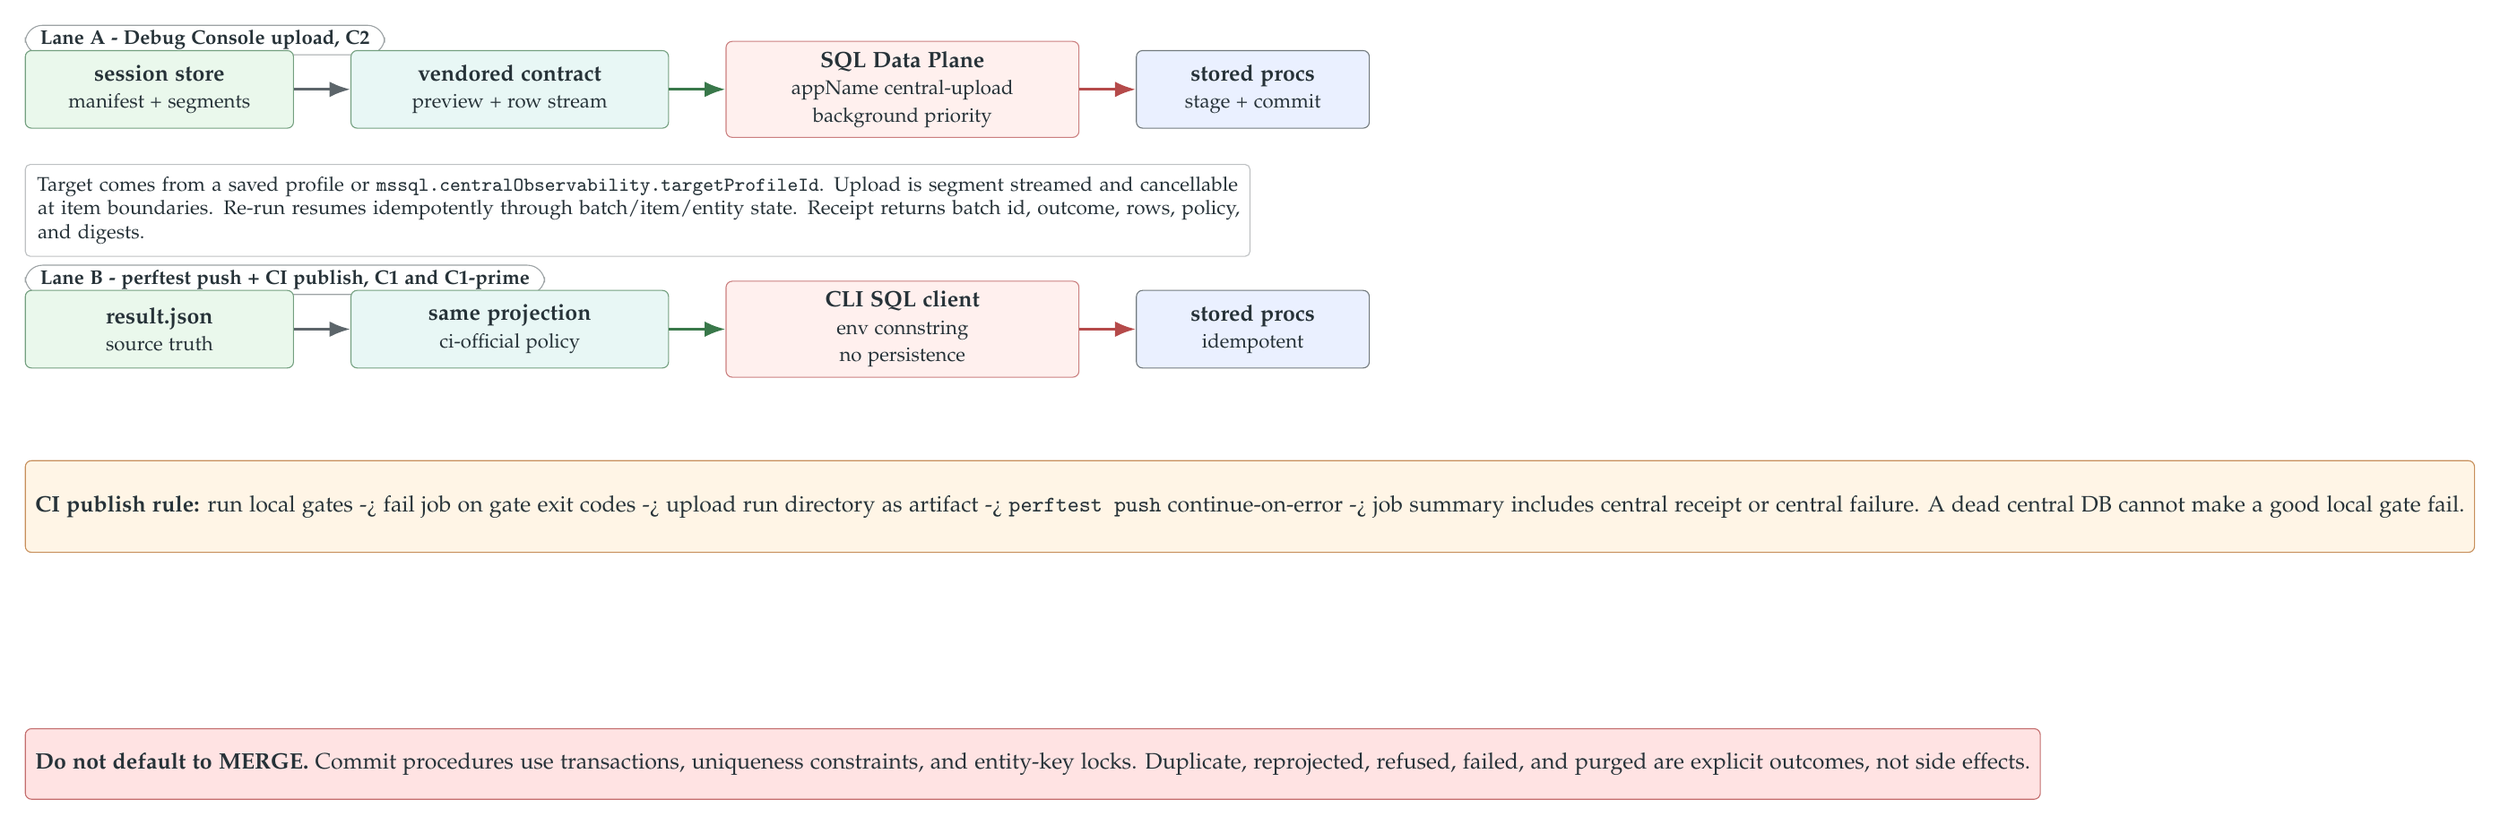
\begin{tikzpicture}[node distance=7mm and 8mm]

\node[pill] (laneA) {Lane A - Debug Console upload, C2};
\node[sourcebox,minimum width=38mm,below=7mm of laneA.west,anchor=west] (a1) {\textbf{session store}\\\footnotesize manifest + segments};
\node[policybox,minimum width=45mm,right=of a1] (a2) {\textbf{vendored contract}\\\footnotesize preview + row stream};
\node[writerbox,minimum width=50mm,right=of a2] (a3) {\textbf{SQL Data Plane}\\\footnotesize appName central-upload\\\footnotesize background priority};
\node[box,minimum width=33mm,right=of a3] (a4) {\textbf{stored procs}\\\footnotesize stage + commit};
\draw[arrow] (a1) -- (a2);
\draw[policyarr] (a2) -- (a3);
\draw[write] (a3) -- (a4);

\node[note,below=5mm of a1.south west,anchor=north west,text width=170mm]
{Target comes from a saved profile or \code{mssql.centralObservability.targetProfileId}. Upload is segment streamed and cancellable at item boundaries. Re-run resumes idempotently through batch/item/entity state. Receipt returns batch id, outcome, rows, policy, and digests.};

\node[pill,below=34mm of laneA.west,anchor=west] (laneB) {Lane B - perftest push + CI publish, C1 and C1-prime};
\node[sourcebox,minimum width=38mm,below=7mm of laneB.west,anchor=west] (b1) {\textbf{result.json}\\\footnotesize source truth};
\node[policybox,minimum width=45mm,right=of b1] (b2) {\textbf{same projection}\\\footnotesize ci-official policy};
\node[writerbox,minimum width=50mm,right=of b2] (b3) {\textbf{CLI SQL client}\\\footnotesize env connstring\\\footnotesize no persistence};
\node[box,minimum width=33mm,right=of b3] (b4) {\textbf{stored procs}\\\footnotesize idempotent};
\draw[arrow] (b1) -- (b2);
\draw[policyarr] (b2) -- (b3);
\draw[write] (b3) -- (b4);

\node[cibox,minimum width=170mm,minimum height=13mm,below=13mm of b1.south west,anchor=north west]
{\textbf{CI publish rule:} run local gates -> fail job on gate exit codes -> upload run directory as artifact -> \code{perftest push} continue-on-error -> job summary includes central receipt or central failure. A dead central DB cannot make a good local gate fail.};

\node[riskbox,minimum width=170mm,minimum height=10mm,below=5mm of b1.south west,anchor=north west,yshift=-46mm]
{\textbf{Do not default to MERGE.} Commit procedures use transactions, uniqueness constraints, and entity-key locks. Duplicate, reprojected, refused, failed, and purged are explicit outcomes, not side effects.};

\end{tikzpicture}
\end{adjustbox}

\newpage
% =====================================================================
% PAGE 6
% =====================================================================
\pagehead{P6. Readers, operations, and retention}
{The central store is useful only if it is queryable, safe to operate, and honest about empty/error/filtered states.}
\legend\par\vspace{4mm}

\begin{adjustbox}{max width=\linewidth,max height=0.82\textheight,center}
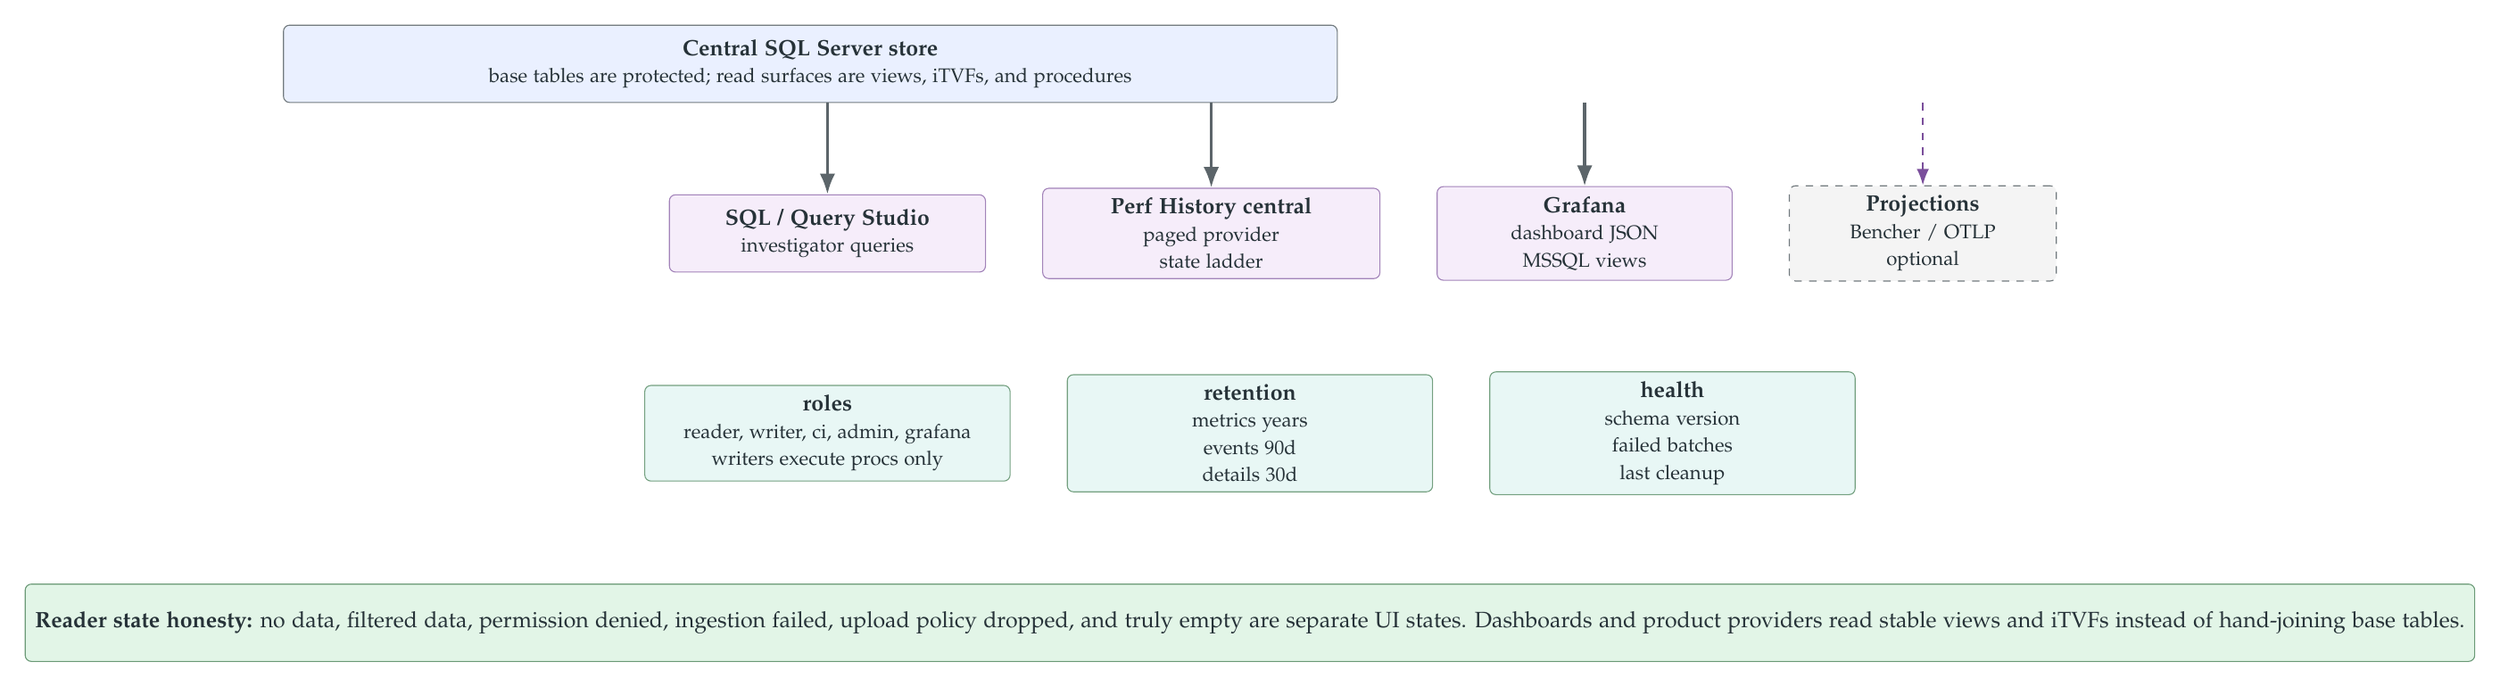
\begin{tikzpicture}[node distance=8mm and 8mm]

\node[box,minimum width=150mm] (store) {\textbf{Central SQL Server store}\\\footnotesize base tables are protected; read surfaces are views, iTVFs, and procedures};

\node[readerbox,minimum width=45mm,below left=13mm and -25mm of store.south] (sql) {\textbf{SQL / Query Studio}\\\footnotesize investigator queries};
\node[readerbox,minimum width=48mm,right=8mm of sql] (ph) {\textbf{Perf History central}\\\footnotesize paged provider\\\footnotesize state ladder};
\node[readerbox,minimum width=42mm,right=8mm of ph] (graf) {\textbf{Grafana}\\\footnotesize dashboard JSON\\\footnotesize MSSQL views};
\node[extbox,minimum width=38mm,right=8mm of graf] (proj) {\textbf{Projections}\\\footnotesize Bencher / OTLP\\\footnotesize optional};

\draw[arrow] (store.south -| sql.north) -- (sql.north);
\draw[arrow] (store.south -| ph.north) -- (ph.north);
\draw[arrow] (store.south -| graf.north) -- (graf.north);
\draw[async] (store.south -| proj.north) -- (proj.north);

\node[policybox,minimum width=52mm,below=16mm of sql] (roles) {\textbf{roles}\\\footnotesize reader, writer, ci, admin, grafana\\\footnotesize writers execute procs only};
\node[policybox,minimum width=52mm,right=of roles] (retention) {\textbf{retention}\\\footnotesize metrics years\\\footnotesize events 90d\\\footnotesize details 30d};
\node[policybox,minimum width=52mm,right=of retention] (health) {\textbf{health}\\\footnotesize schema version\\\footnotesize failed batches\\\footnotesize last cleanup};

\node[goodbox,minimum width=168mm,minimum height=11mm,below=13mm of retention]
{\textbf{Reader state honesty:} no data, filtered data, permission denied, ingestion failed, upload policy dropped, and truly empty are separate UI states. Dashboards and product providers read stable views and iTVFs instead of hand-joining base tables.};

\end{tikzpicture}
\end{adjustbox}

\newpage
% =====================================================================
% PAGE 7
% =====================================================================
\pagehead{P7. Build plan and review decisions}
{Start with C0 contract/schema. Product UI upload waits until projection fixtures and central DDL are green.}
\legend\par\vspace{4mm}

\begin{adjustbox}{max width=\linewidth,max height=0.82\textheight,center}
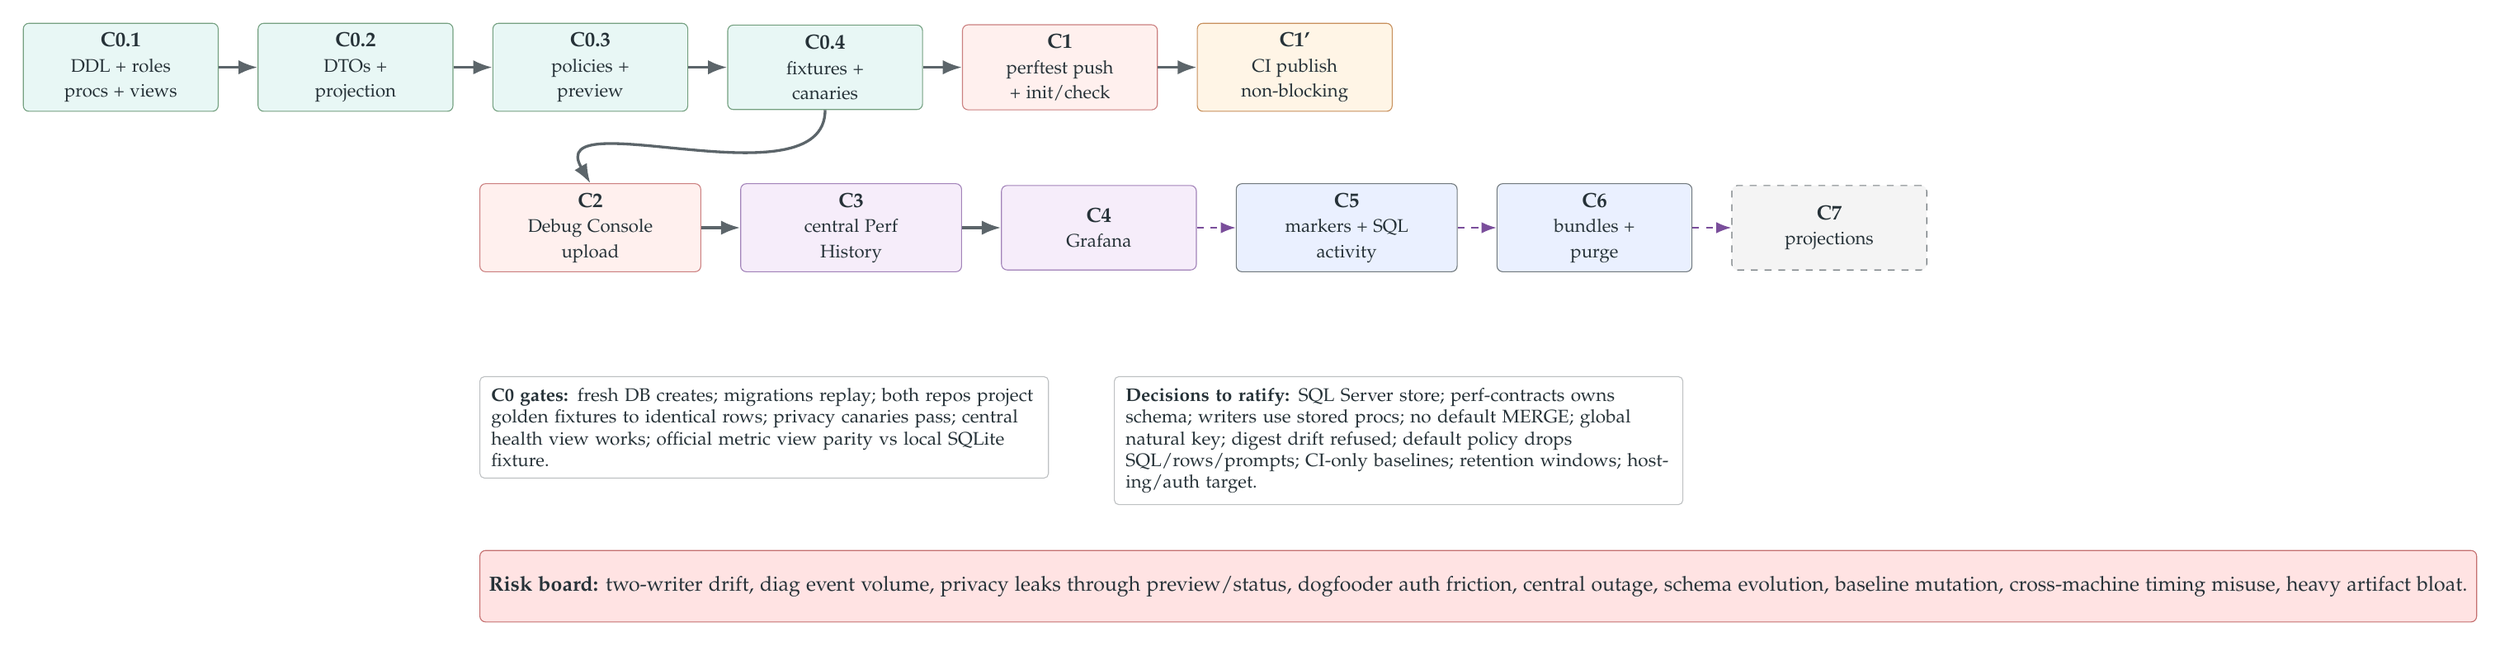
\begin{tikzpicture}[node distance=5mm and 6mm]

\node[policybox,minimum width=30mm,minimum height=13mm] (c01) {\textbf{C0.1}\\\footnotesize DDL + roles\\\footnotesize procs + views};
\node[policybox,minimum width=30mm,minimum height=13mm,right=of c01] (c02) {\textbf{C0.2}\\\footnotesize DTOs +\\\footnotesize projection};
\node[policybox,minimum width=30mm,minimum height=13mm,right=of c02] (c03) {\textbf{C0.3}\\\footnotesize policies +\\\footnotesize preview};
\node[policybox,minimum width=30mm,minimum height=13mm,right=of c03] (c04) {\textbf{C0.4}\\\footnotesize fixtures +\\\footnotesize canaries};
\node[writerbox,minimum width=30mm,minimum height=13mm,right=of c04] (c1) {\textbf{C1}\\\footnotesize perftest push\\\footnotesize + init/check};
\node[cibox,minimum width=30mm,minimum height=13mm,right=of c1] (c1p) {\textbf{C1'}\\\footnotesize CI publish\\\footnotesize non-blocking};

\node[writerbox,minimum width=34mm,minimum height=13mm,below=11mm of c03] (c2) {\textbf{C2}\\\footnotesize Debug Console\\\footnotesize upload};
\node[readerbox,minimum width=34mm,minimum height=13mm,right=of c2] (c3) {\textbf{C3}\\\footnotesize central Perf\\\footnotesize History};
\node[readerbox,minimum width=30mm,minimum height=13mm,right=of c3] (c4) {\textbf{C4}\\\footnotesize Grafana};
\node[box,minimum width=34mm,minimum height=13mm,right=of c4] (c5) {\textbf{C5}\\\footnotesize markers + SQL\\\footnotesize activity};
\node[box,minimum width=30mm,minimum height=13mm,right=of c5] (c6) {\textbf{C6}\\\footnotesize bundles +\\\footnotesize purge};
\node[extbox,minimum width=30mm,minimum height=13mm,right=of c6] (c7) {\textbf{C7}\\\footnotesize projections};

\draw[arrow] (c01) -- (c02);
\draw[arrow] (c02) -- (c03);
\draw[arrow] (c03) -- (c04);
\draw[arrow] (c04) -- (c1);
\draw[arrow] (c1) -- (c1p);
\draw[arrow] (c04.south) to[out=-90,in=120] (c2.north);
\draw[arrow] (c2) -- (c3);
\draw[arrow] (c3) -- (c4);
\draw[async] (c4) -- (c5);
\draw[async] (c5) -- (c6);
\draw[async] (c6) -- (c7);

\node[note,below=16mm of c2.south west,anchor=north west,text width=84mm] (p7note1)
{\textbf{C0 gates:} fresh DB creates; migrations replay; both repos project golden fixtures to identical rows; privacy canaries pass; central health view works; official metric view parity vs local SQLite fixture.};

\node[note,right=10mm of p7note1.north east,anchor=north west,text width=84mm] (p7note2)
{\textbf{Decisions to ratify:} SQL Server store; perf-contracts owns schema; writers use stored procs; no default MERGE; global natural key; digest drift refused; default policy drops SQL/rows/prompts; CI-only baselines; retention windows; hosting/auth target.};

\node[riskbox,minimum width=178mm,minimum height=11mm,below=11mm of p7note1.south west,anchor=north west]
{\textbf{Risk board:} two-writer drift, diag event volume, privacy leaks through preview/status, dogfooder auth friction, central outage, schema evolution, baseline mutation, cross-machine timing misuse, heavy artifact bloat.};

\end{tikzpicture}
\end{adjustbox}

\end{document}
